\section{正の winding 模型の compact fibers と分岐}
\label{pw:section}

第\ref{cw:section}節の正の winding 模型は、他の axes が退化するため、
三つの非退化 focus axes を持つ smooth torus corner の代用にはならない。
しかし、余次元1の分岐を許す構成では、その compact fibers と connected-level quotient を
調べる価値がある。本節では、その quotient を明示計算する。
$x=0$ の有限 isotropy を持つ hyperbolic stratum は局所的な Reeb quotient では分岐を生まない一方、
別の smooth saddle が実際の $Y$ 型分岐を生む。

$\CC^3$ を標準 symplectic form と primitive
$\lambda=\rho_xd\theta_x+\rho_yd\theta_y+\rho_zd\theta_z$ で考え、$c>0$ に対し
\begin{equation}\label{pw:model}
 H=\rho_x+2\rho_y,\qquad J=\rho_y-\rho_z,\qquad
 W=\bar x^2yz,\qquad Q=|W-c|^2
\end{equation}
と置く。角変数の周期は1、$\rho_v=\pi|v|^2$ である。
$W$ は $H,J$ の双方に不変なので、三つの実関数は Poisson commute する。

\subsection{固定した二つの moments による reduction}

まず
\[
 j\ne0,\qquad h>2\max(0,j),\qquad
 L=\max(0,j),\quad U=h/2
\]
を仮定する。$H=h,J=j$ では $u=\rho_y$ を用いて
\begin{equation}\label{pw:radial}
 \rho_x=h-2u,\quad \rho_z=u-j,\quad L\le u\le U,
 \qquad
 f_{h,j}(u)=|W|=\frac{(h-2u)\sqrt{u(u-j)}}{\pi^2}
\end{equation}
と書ける。内部の invariant angle は
\[
 \phi=-2\theta_x+\theta_y+\theta_z\in\RR/\ZZ
\]
であり、$W=f_{h,j}(u)e^{2\pi i\phi}$ となる。

\begin{proposition}[二枚の radial branches]
\label{pw:reduction}
$T^2$-reduced space は、下極 $u=L$ が smooth、上極 $u=U$ が order $2$ の orbifold point
である topological sphere である。内部の symplectic form は
\[
 \omega_{\rm red}=du\wedge d\phi.
\]
$f=f_{h,j}$ は内部にただ一つの critical point
\begin{equation}\label{pw:maximum-point}
 u_0=\frac{h+3j+\sqrt{h^2-2hj+9j^2}}8
\end{equation}
を持ち、それは strict maximum である。$F=F(h,j)=f(u_0)$ と置くと、
$W$ は各 hemisphere $L\le u\le u_0$、$u_0\le u\le U$ を
closed disk $\{|W|\le F\}$ へ homeomorphically 写す。
二つの disk は $|W|=F$ に沿って貼り合わされる。
\end{proposition}

\begin{proof}
$T^2$-action の三つの weights は $(1,0),(2,1),(0,-1)$ である。
内部では action は free で、$\phi$ は primitive な quotient angle となる。
下極では $y$ または $z$ の一方だけが零であり、残る二つの weights の determinant は
$\pm1$ なので smooth である。上極では $x=0$、$y,z\ne0$ であり、
stabilizer は $(s,t)=(1/2,0)$ が生成する $\ZZ/2$ である。
その symplectic slice への作用は $x\mapsto-x$ である。
Cylinder $(L,U)\times S^1$ の両端の circle がそれぞれ点へ潰れるので、
underlying space は sphere となる。
Moment level に標準 form を制限すれば
\[
 (-2du)\wedge d\theta_x+du\wedge d\theta_y+du\wedge d\theta_z
       =du\wedge d\phi
\]
を得る。

内部では
\[
 (\log f)'=-\frac2{h-2u}+\frac1{2u}+\frac1{2(u-j)},\qquad
 (\log f)''=-\frac4{(h-2u)^2}-\frac1{2u^2}-\frac1{2(u-j)^2}<0.
\]
第一の導関数は下端で $+\infty$、上端で $-\infty$ なので、零点は一つである。
その方程式は $8u^2-(2h+6j)u+hj=0$ であり、内部の解が
式\eqref{pw:maximum-point}である。従って $f$ は一方の hemisphere で strictly increasing、
他方で strictly decreasing となる。この radial monotonicity と angle $\phi$ から最後の記述を得る。
\end{proof}

\subsection{有限 isotropy を持つ hyperbolic 極は分岐しない}

\begin{proposition}[上極での Reeb valence]
\label{pw:orbifold-valence}
上極 $u=U$ は $Q=c^2$ の hyperbolic critical point であるが、
その小さい neighborhood の connected-level quotient における valence は $2$ である。
$F\ne2c$ なら global Reeb quotient でも上極の像は valence $2$ である。
$F=2c$ では、上極の像は後述の smooth saddle と同じ vertex になり、
その global valence は $3$ となる。
従ってこの極自身は新たな $Y$ 型分岐を作らない。
\end{proposition}

\begin{proof}
上極近くでは $y,z$ の phases を orbit に沿って固定でき、残る曖昧さは $x\mapsto-x$ である。
$A=\sqrt{U(U-j)}/\pi>0$ とすると uniformizer 上で
\[
 W=A\bar x^2+O(|x|^4),\qquad
 Q-c^2=-2cA\operatorname{Re}(\bar x^2)+O(|x|^4).
\]
従って slice 上では nondegenerate hyperbolic quadratic を持つ。
その二つの positive branches は $x\mapsto-x$ によって交換され、
二つの negative branches も同様に交換される。

より直接には、命題\ref{pw:reduction}より、上極の underlying topological neighborhood で
$W$ 自身が local coordinate である。
その座標で $Q=|W-c|^2$ は $W=0$ において regular なので、level sets は一本の arc となる。
従って局所的な connected-level quotient は interval であり、valence は $2$ である。
後述の critical-point 計算により、同じ $q=c^2$ に他の critical point があるのは $F=2c$ の場合だけである。
その場合、同じ connected level が上極と smooth saddle の双方を含むため、
global quotient では二点の像が一つの三価 vertex に一致する。
それ以外では global quotient の上極の像も valence $2$ である。
\end{proof}

これは元の fiber の smoothness を意味しない。
固定した $(H,J)$-level 内で、上極に対応する singular $T^2$-orbit の近傍は、slice theorem の記法で
\[
 (T^2\times\CC)/\langle(g,x)\mapsto(g+(1/2,0),-x)\rangle
\]
と書ける。Critical slice level は交差する四本の rays であり、その opposite rays が交換される。
Regular orbit から singular orbit への limiting covering は degree $2$ である。
従って Reeb graph に枝がなくても、singular torus fibration とその integral cycle data は残る。

\subsection{内部の smooth saddle と実際の $Y$ 型分岐}

\begin{theorem}[Connected-level quotient の分類]
\label{pw:reeb}
$j\ne0$ と上の moment inequalities を仮定する。
固定した $h,j$ の reduced function $Q$ の Reeb quotient は次の通りである。
\begin{enumerate}
\item $F<c$ なら interval であり、minimum と maximum の値は
 $(c-F)^2,(c+F)^2$ である。内部の generic level は connected circle である。
\item $F>c$ なら $Y$ 型 graph である。二つの minima は $Q=0$ にあり、
 一つの smooth saddle
 \begin{equation}\label{pw:saddle-value}
 q_s=(F-c)^2
 \end{equation}
 で二つの branches が一つに合流する。Maximum は $q_M=(F+c)^2$ である。
 $0<q<q_s$ の generic level は二つの circles、$q_s<q<q_M$ では一つの circle となる。
\item $F=c$ では $Q=0$ に quartic direction を持つ degenerate minimum があり、
 Reeb quotient は interval である。
\end{enumerate}
いずれの場合も、命題\ref{pw:orbifold-valence}の $q=c^2$ は graph の枝を追加しない。
$F=2c$ では smooth saddle と orbifold critical point の値が一致するので、
二つの singularities を別々に扱う際にはこの parameter wall を避ける。
\end{theorem}

\begin{proof}
内部では
\[
 Q=c^2+f(u)^2-2cf(u)\cos(2\pi\phi),\quad
 Q_u=2f'(f-c\cos(2\pi\phi)),\quad
 Q_\phi=4\pi cf\sin(2\pi\phi).
\]
$\phi=1/2,u=u_0$ は唯一の maximum であり、その Hessian の diagonal entries は
$2f''(u_0)(F+c)<0$ と $-8\pi^2cF<0$ である。
$\phi=0,u=u_0$ では、それらが $2f''(u_0)(F-c)$ と $8\pi^2cF$ になる。
従って $F>c$ なら saddle、$F<c$ なら minimum である。
$F>c$ のときはさらに $f(u)=c$, $\phi=0$ に二つの minima があり、
Hessian の diagonal entries は $2f'(u)^2>0$, $8\pi^2c^2>0$ となる。
$F=c$ では $v=u-u_0$ に関して $f-c=\frac12f''(u_0)v^2+O(v^3)$ なので、
$Q$ の leading terms は $\frac14f''(u_0)^2v^4+4\pi^2c^2\phi^2$ である。
下極では $W$ は smooth local coordinate であり、$Q=c^2$ は regular である。
上極の扱いは命題\ref{pw:orbifold-valence}による。

Connected components は double-disk description から直接数えられる。
$F>c$ かつ $\sqrt q<F-c$ なら circle $|W-c|=\sqrt q$ は disk $|W|<F$ の内部にあり、
二つの hemispheres にそれぞれ一つの lift を持つ。
Circle が $|W|=F$ と二点で交わる場合には、disk 内の一つの arc の二つの lifts が両端で貼り合わされ、
一つの circle となる。
$q=q_s$ はこの二つの circles が一点で接する level であり、figure eight となる。
$F<c$ の nonempty regular levels は常に後者の arc の場合である。
これが述べた Reeb graphs を与える。
\end{proof}

\begin{corollary}[全 fibers の compactness と torus components]
\label{pw:compact}
写像 $(H,J,Q):\CC^3\to\RR^3$ は proper である。
上の generic reduced circle の lift は一つの $T^3$ であり、
$F>c$ の saddle 前後では二つの compact $T^3$ components が一つへ合流する。
$F\ne2c$ の smooth saddle fiber は topologically
\[
 T^2\times(S^1\vee S^1)
\]
である。従って connected components of fibers を点へ潰した quotient は、
この saddle locus に沿って実際に余次元1の分岐を持つ。
特に $j\ne0$, $F>2c$ の十分小さい二次元 parameter disk $V$ 上では、
saddle locus の quotient neighborhood は $V\times\mathsf Y$ と同相である。
ここで $\mathsf Y$ は三価 vertex の小さい graph neighborhood を表す。
\end{corollary}

\begin{proof}
Compact な target set 上では $H$ は上に有界、$J$ は下に有界である。
従って $\rho_x\le H$, $\rho_y\le H/2$, $\rho_z=\rho_y-J$ は全て有界となる。
Preimage は closed なので compact である。

Orbifold pole を避ける reduced regular circle の上で $T^2$-action は free であり、
その lift は principal $T^2$-bundle over $S^1$ である。
そのような bundle は trivial なので lift は $T^3$ となる。
$F\ne2c$ なら saddle level は $W=0$ を通らず、action は figure eight 全体でも free である。
Graph 上の principal $T^2$-bundle も trivial なので、最後の表示を得る。
Regular fibers が Lagrangian であることは三つの関数の可換性と dimension から従う。
$F>2c$ では $q_s>c^2$ なので、parameter disk を縮めれば saddle の近くで
orbifold critical level と一様に離れている。
Nondegenerate saddle と二つの radial branches は parameters に滑らかに依存するため、
その connected-level quotient は $V\times\mathsf Y$ となる。
\end{proof}

\subsection{$j=0$ の下 branch にある compact focus block}

\begin{figure}[htbp]
\centering
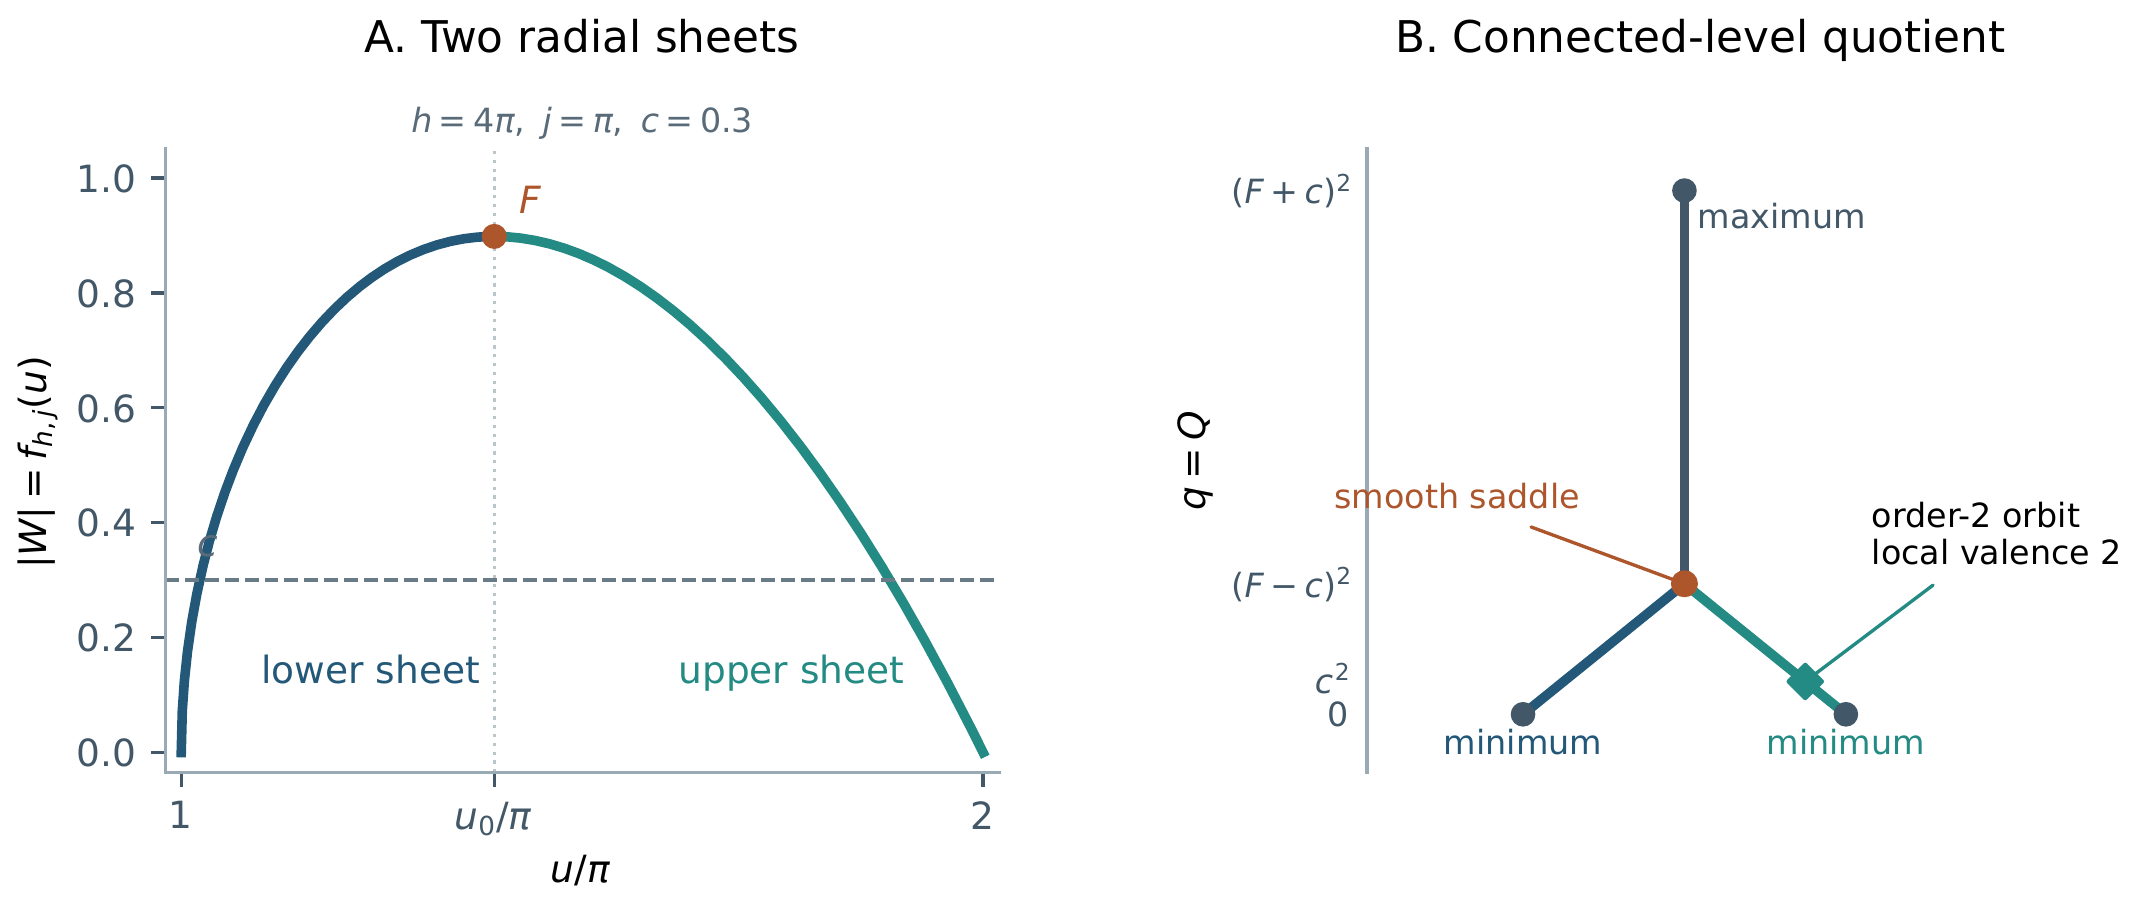
\includegraphics[width=\linewidth]{positive_winding_geometry.png}
\caption{$h=4\pi$, $j=\pi$, $c=0.3$ の例。左は二枚の radial sheets を与える
$f_{h,j}$、右は $Q$ の connected-level quotient である。
この例では $F>2c$ であり、$q=(F-c)^2$ の smooth saddle が真の三価分岐を生む。
$q=c^2$ の order-two orbit は上側の sheet にある singular orbit だが、
その局所 Reeb valence は2である。図の縦座標は実際の critical values を用いている。}
\label{pw:figure}
\end{figure}

上の generic reduction は $j\ne0$ を仮定したが、下 branch の focus fiber は
$x\ne0$ の exact coordinates で直接扱える。
\begin{equation}\label{pw:exact-axis}
 Y=e^{-4\pi i\theta_x}y,\qquad Z=z,
 \qquad
 \lambda=H\,d\theta_x+\rho_Yd\theta_Y+\rho_Zd\theta_Z.
\end{equation}
逆写像は
$x=\sqrt{(H-2\rho_Y)/\pi}\,e^{2\pi i\theta_x}$,
$y=e^{4\pi i\theta_x}Y$, $z=Z$ であり、domain は $H>2\rho_Y$ である。
従ってこれは genuine exact symplectic chart であり、
\begin{equation}\label{pw:axis-family}
 J=\rho_Y-\rho_Z,\qquad
 W=\frac{H-2\rho_Y}{\pi}\,YZ
\end{equation}
が厳密に成り立つ。

\begin{proposition}[分離された compact focus end]
\label{pw:focus}
$h>4\pi\sqrt c$ なら、$(H,J,Q)=(h,0,c^2)$ の fiber は二つの connected components を持つ。
下 branch の component は一つの rank-one focus--focus orbit を持つ
$S^1\times$(once-pinched torus) であり、上 branch の hyperbolic orbit と分離している。
$h$ をこの不等式を満たす compact interval 内で動かせば、
下 branch の全 compact fibers を含む focus curve block を、一様な小さい $(j,q)$-window 上に取れる。
\end{proposition}

\begin{proof}
$j=0$ では $u=\rho_Y=\rho_Z$ であり、
\[
 R=|W|=\frac{(h-2u)u}{\pi^2},\quad
 u_0=h/4,\quad F(h,0)=\frac{h^2}{8\pi^2}.
\]
下 branch の解は
\begin{equation}\label{pw:lower-root}
 u_-(h,R)=\frac{h-\sqrt{h^2-8\pi^2R}}4,
 \qquad 0\le R<F(h,0).
\end{equation}
Node を通る circle $|W-c|=c$ は $0\le R\le2c$ を満たす。
$h>4\pi\sqrt c$ はちょうど $F(h,0)>2c$ なので、
この circle 全体は disk の内部にあり、二つの radial branches の lifts は交わらない。
下 branch では $W=0$ において $Y=Z=0$ の一つの orbit だけが潰れ、
他の点では $J$-orbit は free circle である。
従って $H=h$ で reduction した四次元空間の $(J,Q)$-fiber は once-pinched torus である。
式\eqref{pw:exact-axis}により $\theta_x$ は独立な circle factor なので、元の fiber はその $S^1$ との積である。

原点での quadratic pair は
\[
 J=\pi(|Y|^2-|Z|^2),\qquad
 Q-c^2=-\frac{2ch}{\pi}\operatorname{Re}(YZ)+O(4)
\]
であり、nondegenerate focus--focus 型である。
上 branch の $W=0$ は $x=0$ に対応し、既述の hyperbolic orbit を持つ。
両者の間には $u=u_0$ の positive radial gap がある。
Compact な $h$-interval では $F(h,0)-2c$ が一様に正なので、
$j$ と $q-c^2$ を十分小さくしても二つの branches は分離したままである。
Properness と quotient の一意性により、この下 branch 全体が所要の compact block となる。
\end{proof}

Original disk frames における $x$-axis の mixed coefficient は $-2c\bar x^2$ なので、
削除 disk と逆向きの境界 winding は $+2$ である。
式\eqref{pw:exact-axis}の frame change は $x\ne0$ の annulus 上では well-defined だが、
$x=0$ の disk へは延びない。
従って命題\ref{pw:focus}は、所定の divisor-normal circle を disk まで保つ比較を主張していない。

\begin{corollary}[一次共役因子の smooth-reduction 模型]
\label{pw:m1}
$W_1=\bar x yz$, $H_1=\rho_x+\rho_y$, $J=\rho_y-\rho_z$,
$Q_1=|W_1-c|^2$ と置く。
$j\ne0$, $h>\max(0,j)$ の reduction は両極とも smooth な sphere であり、
$\phi_1=-\theta_x+\theta_y+\theta_z$ に対して $\omega_{\rm red}=du\wedge d\phi_1$ である。
Radial function と唯一の maximum point は
\[
 f_1(u)=\frac{\sqrt{(h-u)u(u-j)}}{\pi^{3/2}},\qquad
 u_1=\frac{h+j+\sqrt{h^2-hj+j^2}}3,
 \qquad \max(0,j)\le u\le h.
\]
$F_1=f_1(u_1)>c$ なら Reeb quotient は $Y$ 型であり、
$q_s=(F_1-c)^2$ の whole saddle fiber は $T^2\times(S^1\vee S^1)$ である。
ここでは $F_1=2c$ を除外する必要はない。
$F_1<c$ と $F_1=c$ の分類も定理\ref{pw:reeb}と同じである。

$j=0$ では
\[
 u_1=2h/3,\qquad F_1(h,0)=\frac{2h^{3/2}}{3\sqrt3\,\pi^{3/2}},
 \qquad F_1(h,0)>2c\ \Longleftrightarrow\ h>3\pi c^{2/3}.
\]
この範囲の $(h,0,c^2)$-fiber は、下側の
$S^1\times$(once-pinched torus) と上側の regular $T^3$ に分離する。
下 component は compact な $h$-interval 上で一様な focus block を与える。
各 nonzero axis の transverse 型は、$x$-axis が focus--focus、
$y,z$-axes が elliptic--elliptic である。
\end{corollary}

\begin{proof}
Weights $(1,0),(1,1),(0,-1)$ の任意の二つは unimodular なので、
$j\ne0$ の moment level では両極を含め action が free である。
また $(\log f_1)''<0$ で、critical equation は
$3u^2-2(h+j)u+hj=0$ となる。
命題\ref{pw:reduction}の double-disk argument と系\ref{pw:compact}の
graph 上の principal bundle の議論を適用できる。
上極では $W_1$ は非零定数倍の $\bar x$ を leading term とする smooth coordinate なので、
$Q_1=c^2$ も regular である。

$x\ne0$ では $Y=e^{-2\pi i\theta_x}y$, $Z=z$ によって厳密に
\[
 \lambda=H_1d\theta_x+\rho_Yd\theta_Y+\rho_Zd\theta_Z,
 \qquad W_1=\sqrt{\frac{H_1-\rho_Y}{\pi}}\,YZ
\]
となる。$j=0$ の lower branch は
$u^2(h-u)=\pi^3R^2$ の $0\le u<2h/3$ の解である。
$F_1>2c$ なら $|W_1-c|=c$ 全体がこの branch に入り、
命題\ref{pw:focus}と同じ積分解と uniform gap の議論が使える。
原点での $(J,Q_1-c^2)$ の quadratic pair は非零係数の $\operatorname{Re}(YZ)$ を持つ focus 型である。
一方、$y$-axis の stabilizer moment は $H_1-J=\rho_x+\rho_z$、
もう一方の quadratic は $-2c\operatorname{Re}(y_0\bar xz)$ である。
Unitary basis によってこの二つを $|v_1|^2,|v_2|^2$ の線形結合へ同時対角化でき、
elliptic--elliptic 型となる。$z$-axis も同様である。
\end{proof}

\begin{remark}[Semistable frames への位相変換]
\label{pw:semistable-phase}
本節の winding $+1,+2$ は original disk frames に関する値である。
第\ref{sc:phase}節の $C_{56}$ の端では、固定した $t\ne0$ に対し $y=tY/x$ なので、
mixed coefficient は
\[
 \gamma_{\rm ss}(x)=\frac{t}{x}\gamma_{\rm orig}(x),\qquad
 \operatorname{wind}_{\rm ss}=\operatorname{wind}_{\rm orig}+1
\]
と変換される。境界は常に削除 disk と逆向きである。
定数 $-2c$ を省略した係数を比較すると、次の表となる。
\[
\begin{array}{c|r|c|r}
 W&\text{original winding}&\gamma_{\rm ss}/(-2c)&\text{semistable winding}\\ \hline
 xyz&-1&t&0\\
 yz&0&t/x&1\\
 \bar xyz&1&t\bar x/x&2\\
 \bar x^2yz&2&t\bar x^2/x&3.
\end{array}
\]
従って系\ref{pw:m1}の模型が、第\ref{sc:phase}節の最大 winding を最小にする配分の
$+2$ の端に対応する候補となる。
$\bar x^2yz$ の模型の $+2$ を、その配分の $+2$ と直接同一視しない。
一方 $\sigma=L_1^3L_2L_3L_4$ を選べば semistable winding は $(3,1,1,1)$ となり、
$6(3+1+1+1)=36$ という別の位相収支も満たせる。

これらは固定した非零 $t$ の annulus 上の phase 計算である。
$t\to0$ で非零 Hessian を残すには、$W/t$ を使うなどの scale の選択を別途指定する必要がある。
またこの表は、actual Kähler form、normal circles、marked actions、whole fibers を保つ
relative symplectic identification を与えるものではない。
\end{remark}

この計算から得る具体的な次の課題は、下 branch の正の winding focus ends、
上 branch の有限 isotropy を持つ singular wall、内部の $Y$ 型 saddle を、
actual semistable geometry の中で相対的に配置することである。
有限 isotropy の wall と他の coordinate axes の退化は、二次共役因子 $\bar x^2yz$ の模型に属する。
その $F>2c$ の領域では focus component と上の singular wall を分離して扱える。
一次共役因子 $\bar xyz$ の模型では、上の component は regular であり、他の axes は elliptic--elliptic となる。
二次模型の $F=2c$ での collision、各模型の $F=c$ の degenerate minimum、
elliptic endpoints と残る axis singularities を含む全 corner の処理は未完了である。
本節は全 corner や boundary-free global fibration の完成ではなく、
compact fibers を保った正の winding と真の余次元1分岐が共存する finite-neck prototype を与える。


第\ref{tp:section}節では、この prototype を chosen graph Kähler form へ実際に移し、
中央の一端と exact に比較する。
第\ref{ai:section}節では、$x=0$ を除いても whole focus と true saddle が残る compact block を取り、
actual annulus へ入れる。従って prototype の位相計算から actual な局所構成へ進めるが、
除いた端と geometric corner 全体の充填は別の問題として残る。
